\subsection{Fundamental definitions}

\begin{definition}{Sequence set}{sequence_set}
  Let \Sequences{} be a set of DNA sequences.
  Each sequence \(s \in \Sequences{}\) is a string of length \(|s|\).
  As a DNA sequence, it can be read in two orientation:
  the forward orientation (original sequence in the set) and the reverse complementary orientation (short in reverse).

  Let \( \Orientations{} = \Set{f, r} \) be the set of sequence orientations (\(f\) for forward and \(r\) for reverse).

  Let \( \OrSeqs{} = \Sequences{} \times \Orientations{} \) be the set of oriented sequences.
  For a sequence \(s \in \Sequences{}\), we can write its associated oriented sequences in \OrSeqs{} \(s_f\) and \(s_r\) for respectively the forward and reverse of \(s\).

  Given \(a \in \OrSeqs{}\), by \(\rev{a}\) we denote the reverse-complementary oriented sequence of \(a\) (by abuse: its reverse).
\end{definition}

\begin{definition}{Link set}{link_set}
  Let \(\Links{} \subset \OrSeqs{}^2\) be a set of links between two oriented sequences in \OrSeqs{}.
  For each \(l = (a, b) \in \Links{}\), the reverse link also exists, i.e.\ \(\rev{l} = (\rev{b}, \rev{a}) \in \Links{} \). % chktex 21
\end{definition}

In this paper, we illustrate the sequences and their links with a figure like \zcref[S]{subfig:sequence_graph:artistic_view}.
However, to simplify the future mathematical models, we use the directed graph structure (\zcref[S]{definition:sequence_graph_dg}) as \zcref[S]{subfig:sequence_graph:dg} illustrates.

\begin{definition}{Sequence graph}{sequence_graph_dg}
  Let \(G = (V_{\Sequences{}}, A_{\Links{}})\) be a directed graph where:

  \begin{itemize}
    \item \(V_{\Sequences{}}\) is the vertex set representing the oriented sequences (\(|V_{\Sequences{}}| = |\OrSeqs|\))
    \item \(A_{\Links{}}\) is the set of arcs representing the links (\(|A_{\Links{}}| = |\Links|\))
  \end{itemize}
\end{definition}

\begin{figure}
  \centering
  \begin{subfigure}{0.35\linewidth}
    \centering
    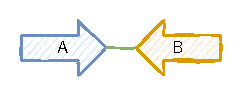
\includegraphics[width=\linewidth]{introduction/img/sequence_graph-figure.pdf}
    \caption{Artistic view}\label{subfig:sequence_graph:artistic_view}
  \end{subfigure}
  \hfill
  \begin{subfigure}{0.35\linewidth}
    \centering
    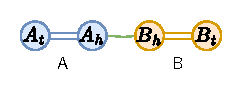
\includegraphics[width=\linewidth]{introduction/img/sequence_graph-UG.pdf}
    \caption{Undirected graph}\label{subfig:sequence_graph:ug}
  \end{subfigure}
  \hfill
  \begin{subfigure}{0.185\linewidth}
    \centering
    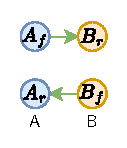
\includegraphics[width=\linewidth]{introduction/img/sequence_graph-DG.pdf}
    \caption{Directed graph}\label{subfig:sequence_graph:dg}
  \end{subfigure}
  %
  \figurecaption{Sequence graph representations}{%
    The three subfigures represent the same informations:
    two sequences \(\mathsf{A}\) (in blue) and \(\mathsf{B}\) (in orange), and a link between them \((\mathsf{A}_f, \mathsf{B}_r)\) (in green).
    %
    \Subref{subfig:sequence_graph:artistic_view}
    %
    The arrows are the oriented sequences, the green line is the link.
    %
    \Subref{subfig:sequence_graph:ug}
    %
    The undirected graph structure visually closer to the artistic view than the directed graph in \subref{subfig:sequence_graph:dg}.
    Each vertex is representing the tail otherwise the head of the arrow, double edges maintain the integrity of the sequences while the simple edge represents the link.
    \zcref[S]{definition:sequence_graph_ug} formally describes the graph structure.
    %
    \Subref{subfig:sequence_graph:dg}
    %
    The directed graph structure is an explicit representation of the oriented sequences and their (oriented) links.
    Each vertex is one sequence in a fixed orientation.
    One link and its reverse are the arcs.
  }\label{fig:sequence_graph}
\end{figure}
